% Adjusting chapter title format for regular (numbered) chapters
\titleformat{\chapter}[display]
  {\normalfont\huge\bfseries\centering}{\chaptertitlename\ \thechapter}{20pt}{\Huge}

% Using similar styling for unnumbered chapters but without "Chapter" prefix
\titleformat{name=\chapter,numberless}
  {\normalfont\huge\bfseries\centering}{}{0pt}{\Huge}

\titlespacing*{\chapter}{0pt}{50pt}{40pt} % Adjust vertical spacing before and after the title


\chapter{Introduction} % Ensures chapter numbering starts correctly
\section{Overview} % This will now be Section 1.1, not 0.1

Deep Neural Networks, or DNNs, are increasingly being
used in diverse applications owing to their ability to match
or exceed human level performance. The availability of large
datasets, fast computing methods and their ability to achieve
good performance has paved way for DNNs into safety-critical
avenues such as autonomous car driving, medical diagnosis,
security, etc. The safety-critical nature of such applications
makes it imperative to adequately test these DNNs before
deployment. However, unlike traditional software, DNNs do
not have a clear control-flow structure. They learn their
decision policy through training on a large dataset, adjusting
parameters gradually using several methods to achieve desired
accuracy. Consequently, traditional software testing methods
like functional coverage, branch coverage, etc. cannot be
applied to DNNs, thereby challenging their use for safety critical applications.
A lot of recent work, discussed in chapter II, has looked into
developing testing frameworks for DNNs. These methods
suffer from certain limitations, as discussed in \hypertarget{challenges}{}. In our work,
we intend to make an effort to overcome these limitations and
build a fast, scalable, efficient, generalizable testing framework for
deep neural networks. 

In this section of thesis, the background and motivation,  \hyperlink{researchquestions}{Research Questions}, \hyperlink{contributions}{contributions} and \hyperlink{organization of thesis}{organization of thesis} have been presented.

\subsection{Background and motivation}

In the past few years, deep neural networks (DNNs) have made remarkable progress in achieving human-level performance. With the broader deployment of DNNs on various safety critical systems like autonomous, healthcare, avionics, etc., the concerns over their safety and trustworthiness have been raised in public, particularly highlighted by incidents involving self-driving cars.

An important low-level requirement for DNNs is that they are robustness against input perturbations. DNNs have been shown to suffer from a lack of robustness because of their susceptibility to adversarial examples such that small modifications to an input, sometimes imperceptible to humans, can make the network unstable.

In this thesis, we examine existing testing methods for
deep neural networks, the opportunities for improvement and
the need for a fast, scalable, generalizable end-to-end testing
method.

Coverage criteria for traditional software programs, such as code coverage and branch coverage check that all parts of the logic in the program have been tested by at least one test input and all conditions have been tested to independently affect the entailing decisions. On similar lines, any coverage criterion for deep neural networks must be able to guarantee completeness, that is, it must be able to ensure that all parts of the internal decision-making structure of the DNN have been exercised by at least one test input.

Generating or selecting test inputs in a guided manner usually has two major goals - maximizing the number of uncovered faults, and maximizing the coverage.
	
Testing DNNs for correctness involves verifying behaviors against a ground truth or oracle. The traditional approach, collecting and manually labeling real-world data, is labor-intensive. Another method compares outputs across multiple DNNs for the same task, identifying discrepancies as corner cases. However, this can misclassify inputs if all models agree, due to shared biases or errors. This comparative approach is further limited to tasks with multiple reliable models, which may not always be available, especially in innovative or specialized applications.



\begin{figure*}[h]
	\centering
	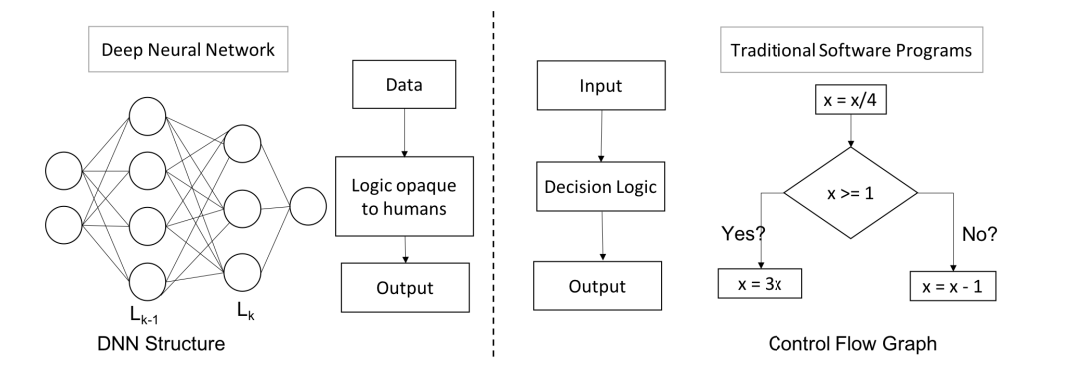
\includegraphics[width=0.8\textwidth]{fig1.png}
	\caption{The internal logic of a deep neural network is opaque
	to humans, as opposed to the well laid out decision logic of
	traditional software programs \cite{Intro_1}}
	\label{fig:1}
\end{figure*}

\begin{figure*}[h]
	\centering
	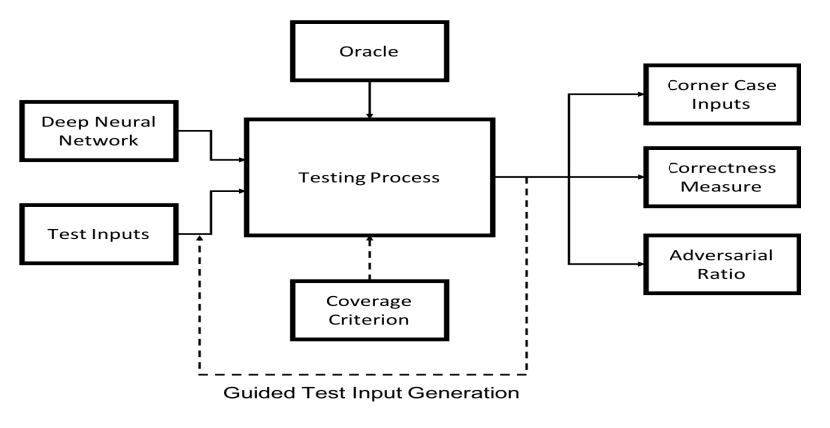
\includegraphics[width=0.8\textwidth]{fig2.png}
	\caption{A high-level representation of most existing DNN
	testing methods \cite{Intro_1}}
	\label{fig:2}
\end{figure*}
	
\subsection{Challenges of Deep Learning Models}
The growing use of deep neural networks in safety critical applications makes it necessary to carry out adequate testing to detect and correct any incorrect behavior for corner case
inputs before they can be actually used. Deep neural networks
lack an explicit control-flow structure, making it impossible to
apply to them traditional software testing criteria such as code
coverage

\begin{itemize}
	% \item existing mechanisms depend on manual collections of labelled data that cause \textbf{unguided simulation}
	\item input space is extremely large, \textbf{unguided simulation} are higly unlikely to find erroneous behavior
   \end{itemize}

\subsection{Challenges in Testing of Deep Learning Models} \hypertarget{challenges}{}
unlike traditional software, DNNs do not have a clear control-flow structure. They learn their decision policy through training on a large dataset, adjusting parameters gradually using several methods to achieve desired accuracy. Consequently, traditional software testing methods like functional coverage, branch coverage, etc. cannot be applied to DNNs, thereby challenging their use for safety- critical applications.Traditional software testing methods fail when applied to DNNs because the code for deep neural networks holds no information about the internal decision-making logic of a DNN.


DNNs testing techniques aim to discover bugs, through finding counter examples that challenge the system's correctness, or to establish confidence by rigorously evaluating the system with numerous test cases. These testing techniques are computationally less expensive and therefore are able to work with state-of-the- art DNNs. However, DL testing has some limitations:
\begin{itemize}
    \item Standards available in industry but \textbf{Lack of Logcial Structure} and \textbf{System Specification}  
     \item Heavily depend on manual collections of test data under different conditions which become expensive as number of test condition increases
     \item  existing coverage criteria are not detailed enough to notice subtle behaviours exhibited by DL systems.
\end{itemize}

coarse coverage criteria, open ended processes, unreliable
oracles, inefficient test input generation methods, inability to
scale to larger DNNs and different network architectures


		
		
\subsection{Research Questions}\hypertarget{researchquestions}{}
\begin{itemize}
	\item How to specify relevant local robustness properties?
	\item How we sample inputs efficiently?
	% \item How to explore input-output space efficiently?
	% \item How to generate realistic input to automate such exploration?
	% \item How to automatically collect create test oracle that detect erroneous behavior?
	\item How to design comprehensive framework?
   \end{itemize}

% Why do we need a better coverage criteria?
% Why do we need better test input generation?
% Why do we need a better oracle?

\subsection{Thesis Contributions}\hypertarget{contributions}{}
The idea is to propose coverage criteria to evaluate the adequacy of test inputs. A good test input should be surprising enough to challenge the system, revealing behaviors not seen during training, but not so surprising that it becomes irrelevant or unrealistic compared to the training data.

a test case generation method is proposed to generate test inputs that have greater coverage and which uncover greater corner case behavior.
\begin{itemize}	
	\item abc
\end{itemize}


\subsection{Organization of thesis}\hypertarget{organization of thesis}{}
The remainder of the thesis is organized as follows: related studies are presented in Chapter \ref{chp:2}. System model and proposed methodology are demonstrated in Chapter \ref{chp:3}. Chapter \ref{chp:4} describes the simulation results of our proposed schemes. Finally, the findings of this work along with future directions are presented in Chapter \ref{chp:6}.


\clearpage
